\chapter{Pesquisa de Mercado}
%TODO: jpg é pessimo para texto. Usar png quando possível, ou um arquivo vetorizado (pdf, ps, eps...).
%TODO: citar fonte das figuras
\label{mercado}
Segundo pesquisa da \emph{International Air Transport Association} (IATA) o número de passageiros esperado em 2036 é de 7.8 bilhões, quase o dobro do número de passageiros esperado para esse ano (4 bilhões).
Portanto, o mundo precisa se preparar para dobrar o número de passageiros dentro de 20 anos. \cite{iata}

O esperado é que o mercado chinês vai superar o mercado aeronáutico dos Estados Unidos, como sendo o maior mercado de passageiros (definido pelo tráfego partindo e dentro do país), até 2030.
Isso ocorrerá devido à combinação de uma taxa de crescimento mais rápida do mercado chinês com a redução da taxa de crescimento do mercado americano. (Veja a \autoref{fig:major-domestic-markets}.) \cite{iata}

\begin{figure}[H]
\centering
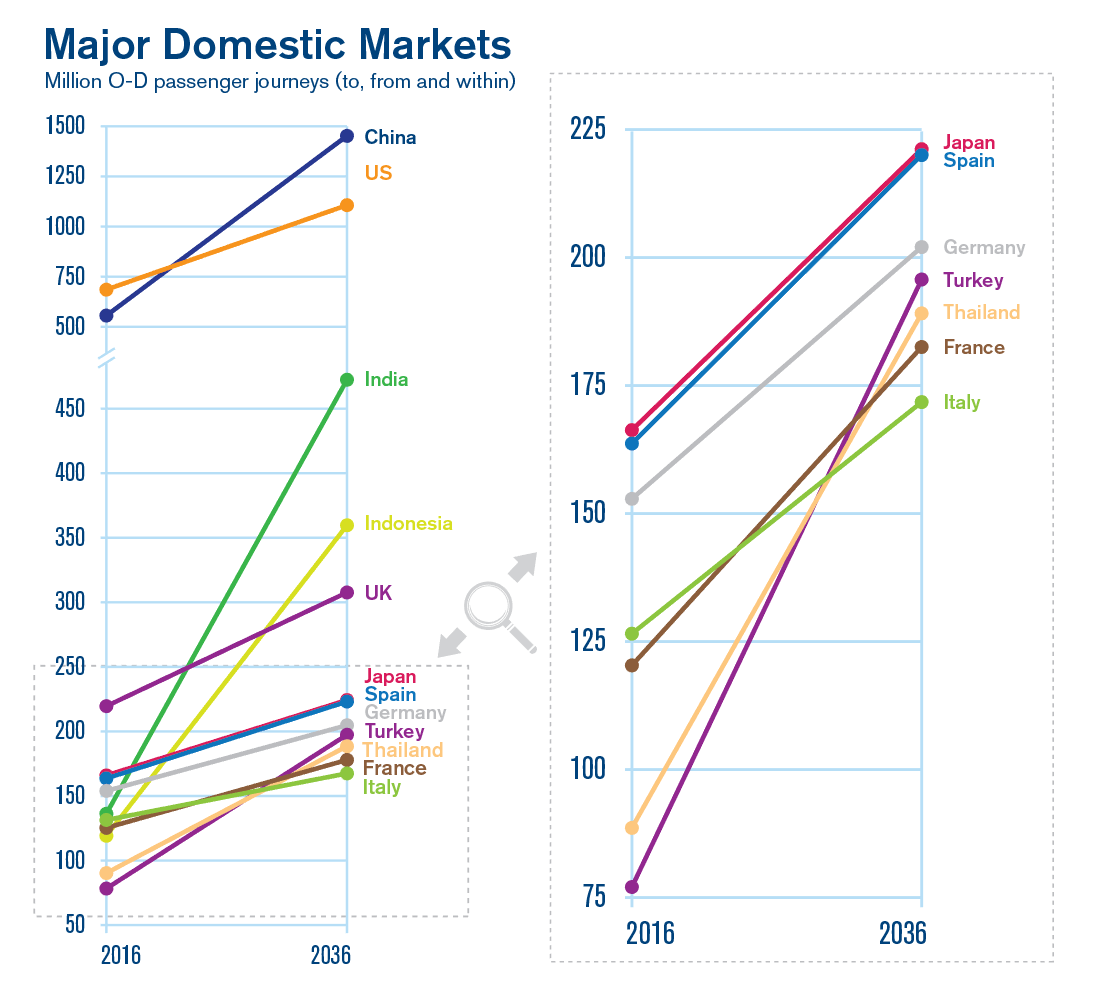
\includegraphics[width=0.75\textwidth]{pesquisademercado/major-domestic-markets.png}
\caption[Perspectiva de crescimento dos mercados domésticos até 2036]{Perspectiva de crescimento dos mercados domésticos até 2036\cite{iata}.}
\label{fig:major-domestic-markets}
\end{figure}

Como pode ser percebido no gráfico acima, ambos os mercados permanecerão como sendo os maiores do mundo com uma grande margem em relação aos outros.
A tendência esperada é a de que os Estados Unidos permanecerá sendo o maior mercado de passageiros aéreos até por volta de 2030, quando seguirá para a segunda posição atrás do mercado chinês.
Portanto, para a realização da pesquisa de mercado de projeto desenvolvido, foram levados em conta os mercados americano e chinês. 
Como o mercado americano aeronáutico é o maior atualmente e sabendo que, dentro de vinte anos, ele permanecerá no topo da lista, a frota atual de aeronaves desse mercado foi considerada como sendo a mais relevante para a pesquisa de mercado do projeto da nova aeronave.
Veja a \autoref{fig:marketforecast}.

\begin{figure}[H]
\centering
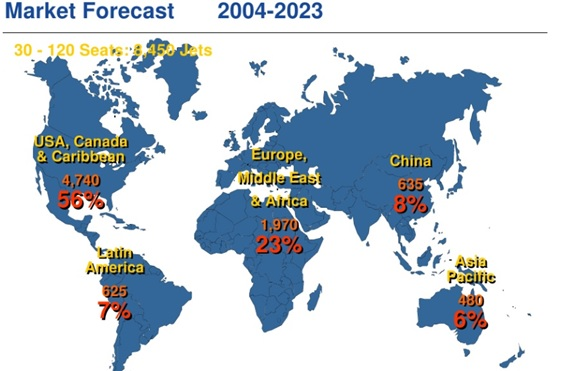
\includegraphics[width=0.75\textwidth]{pesquisademercado/marketforecast.jpg}
\caption[Previsão de mercado para 2004--2023]{Previsão de mercado para aeronaves de 30--120 passageiros entre os anos de 2004 e 2023. Observa-se a dominância do mercado americano neste setor}
\label{fig:marketforecast}
\end{figure}

A aviação regional possui um grande papel no mercado visto que permite que as companhias aéreas forneçam um equilíbrio correto entre a capacidade e a frequência das rotas chaves. Possui um importante papel também ao alimentar as rotas principais dentro de uma determinada região, suplementando, quando necessário, a capacidade das linhas aéreas que voam as rotas principais. Quando o mercado está fraco, a aviação regional pode ser utilizada visando defender a posição da companhia aérea dentro do mercado, mantendo a frequência das rotas, mas com uma capacidade de transportar menor quantidade de passageiros, substituindo uma aeronave de grande porte previamente utilizada para determinada rota. Além disso, uma aeronave regional também permite que as companhias aéreas lidem com a flutuação da demanda em diferentes estações do ano, bem como a flutuação durante o dia. Portanto, com base nas aplicações descritas acima, bem como outras aplicações, percebe-se a importância da aviação regional como sendo uma parte essencial no mercado da aviação mundial.

A aviação regional cresceu firmemente nas duas últimas décadas no mundo e não há indicações para esta tendência abaixar.  Nos Estados Unidos, definido como o principal mercado para o projeto em desenvolvimento, as companhias aéreas da aviação regional possuem vantagens de custos operacionais devido aos tipos de rotas que elas operam, definidos como voos curtos e médios (\emph{short and medium haul}) conectando comunidades menores, em rotas pouco densas, às grandes cidades. Portanto, o mercado da aviação regional, constituído de aeronaves que transportam, na média, de 30 a 70 passageiros, é de relativa importância. 

%Imagem removida porque é muito grande e não relevante, a tabela dos 5 principais concorrentes resume bem a informação.
%TODO: citar essa tabela no texto
%\begin{table}
%\centering
%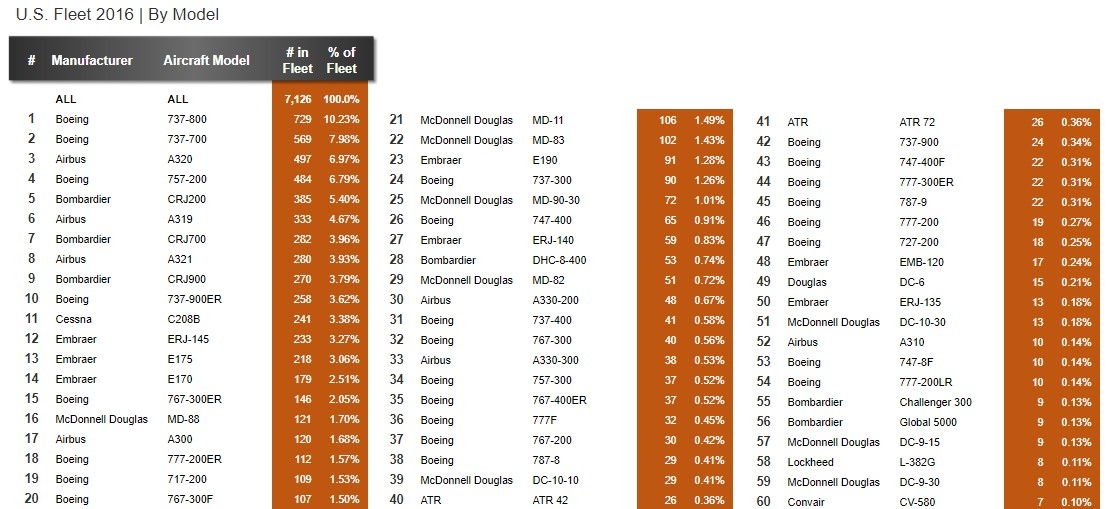
\includegraphics[width=\textwidth]{pesquisademercado/fleet.jpg}
%\caption{Número de aeronaves por modelo na frota de aeronaves dos Estados Unidos em 2016.}
%\label{fig:fleet}
%\end{table}

\begin{table}[bt]
\centering
\begin{tabular}{llr}
\toprule
Fabricante & Modelo & Quantidade\textsuperscript{$\dagger$} \\ \midrule
Bombardier & CRJ200 & 385 \\
Embraer    & ERJ145	& 233 \\
Embraer    & E170	& 179 \\
Bombadier  & Dash 8 Q400 & 53 \\
ATR		   & ATR 42 & 26 \\
Embraer    & E120   & 17 \\
\bottomrule
\end{tabular}

{\footnotesize\textsuperscript{$\dagger$}Número de aeronaves na frota dos Estados Unidos no ano de 2016.}
\caption[Principais concorrentes]{Principais concorrentes: aeronaves com capacidade de 30--100 passageiros mais vendidas no mercado americano.\cite{fiaeroweb}}
\label{tbl:maisvendidas}
\end{table}

As aeronaves listadas na 
 \autoref{tbl:maisvendidas} foram consideradas como sendo os principais competidores do projeto em desenvolvimento pela equipe.


\section{Principais Concorrentes}
    Entre as configurações de projeto, especialmente voltada para a aviação regional, o CRJ200 apresenta um design avançado das asas, turbofans de alta eficiência, capacidade adicional de combustível e um teto de serviço certificado mais alto (41000ft). Em relação à performance, possui um alcance de 1650nm, sendo o terceiro maior alcance dentre as aeronaves analisadas, e uma velocidade de cruzeiro de 424kts. O custo estimado de operação desta aeronave é de 1104 doláres por hora. 
	
    A segunda aeronave mais vendida na categoria analisada é a ERJ145, um turbo jato desenvolvido pela Embraer no final do século passado, é a que possui a maior velocidade de cruzeiro (450kts) dentre as analisadas e possui um alcance de 1320nm. O seu custo operacional estimado é o segundo mais baixo, sendo aproximadamente 846 doláres por hora, ficando atrás somente da aeronave E170, que é uma aeronave relativamente maior que as outras. Esta aeronave opera em um teto de serviço de 41000ft, tem um alcance de 2150nm, o segundo maior, e possui o terceiro maior número de aeronaves entregues dentre as analisadas. 
	
    A quarta aeronave mais vendida da categoria é a Dash-8, que possui um alcance de 1100nm, opera em um teto de 27000ft e o segundo maior custo operacional por hora de 1313 doláres. Com base na análise de mercado, em quinto lugar no número de aeronaves vendidas tem o ATR-42, que possui o custo mais alto de operação de 1552 doláres por hora, isto se deve principalmente pelo fato de ser uma aeronave mais antiga. No entanto, esta aeronave tem a vantagem de possuir o maior alcance dentre os modelos analisados, sendo igual a 2720nm. E a última aeronave analisada em mais detalhes foi a EMB120, que possui um custo operacional por hora relativamente alto, de 1313 doláres, e o menor alcance de 945nm. 
    
    As figuras nas páginas seguintes contém dados básicos, e seções em corte dessas aeronaves.

\clearpage
%\subsection{Bombardier CRJ 200}

\begin{figure}[bp]
\centering
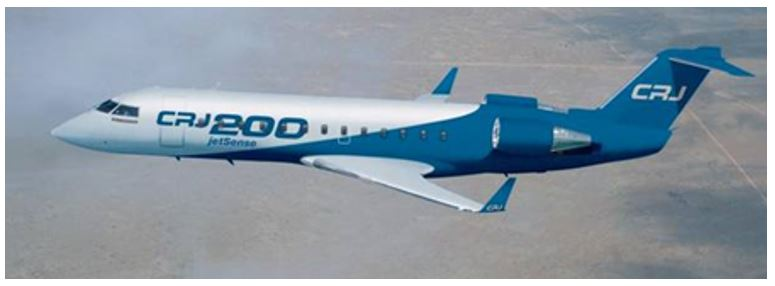
\includegraphics[width=1\textwidth]{pesquisademercado/BombardierCRJ200.jpg}
\caption{Bombardier~CRJ200}
\end{figure}

\begin{table}[bp]
\centering
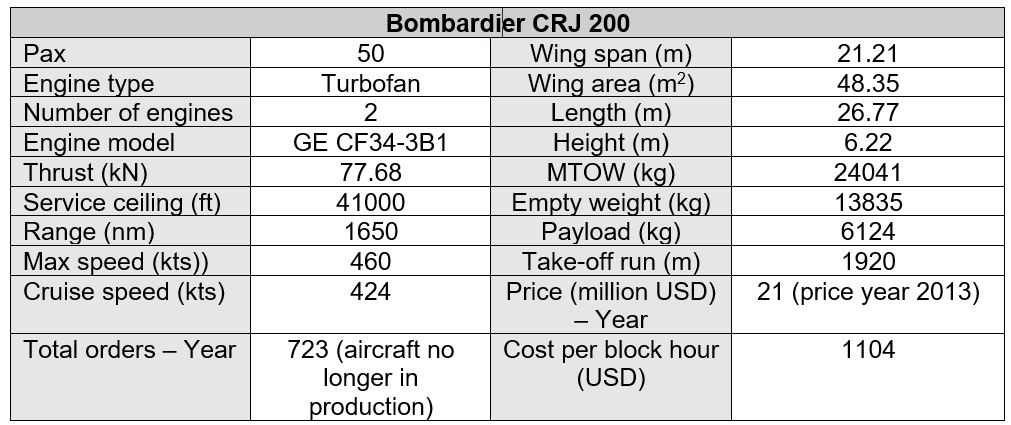
\includegraphics[width=0.9\textwidth]{pesquisademercado/tabelaBombardierCRJ200.jpg}
\caption{Características do Bombardier~CRJ200}
\end{table}

\begin{sidewaysfigure}[p]
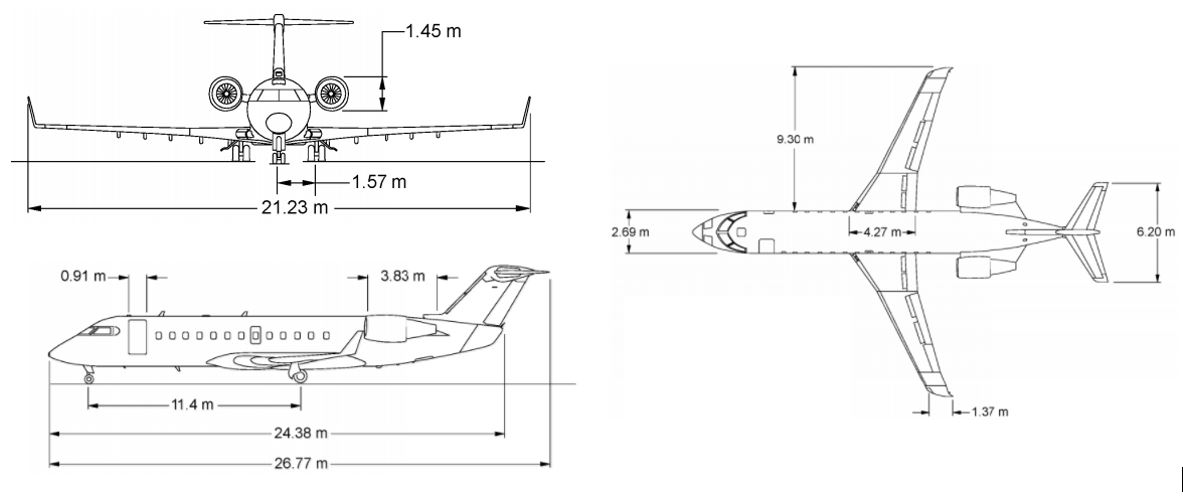
\includegraphics[width=\textwidth]{pesquisademercado/dimensoesExternasBombardierCRJ200.jpg}
\caption{Três vistas do Bombardier~CRJ200}
\end{sidewaysfigure}

\begin{sidewaysfigure}[p]
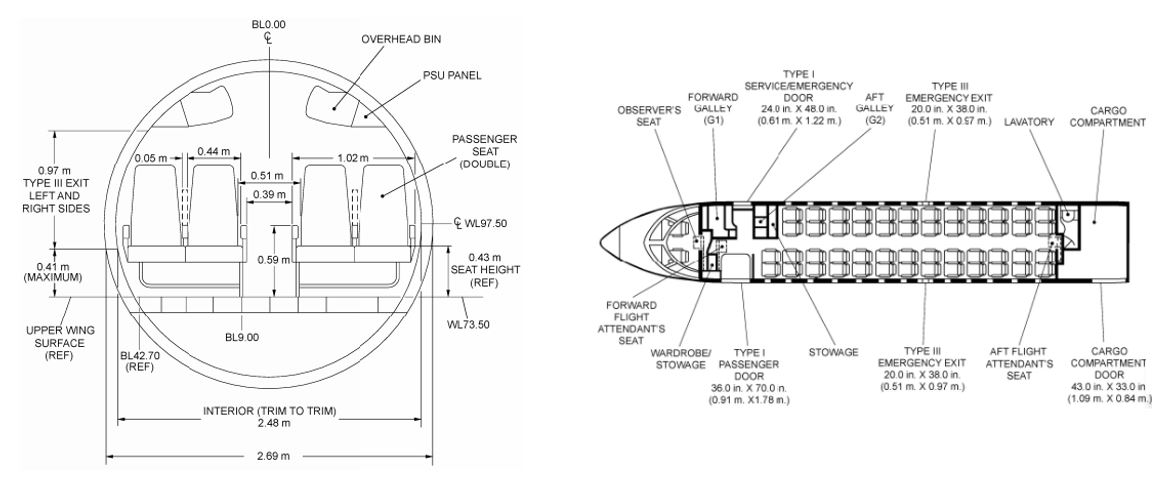
\includegraphics[width=\textwidth]{pesquisademercado/dimensoesInternasBombardierCRJ200.jpg}
\caption{Seção transversal e longitudinal (LOPA) do Bombardier~CRJ200}
\end{sidewaysfigure}

\clearpage
%\subsection{Embraer ERJ 145}
\begin{figure}
\centering
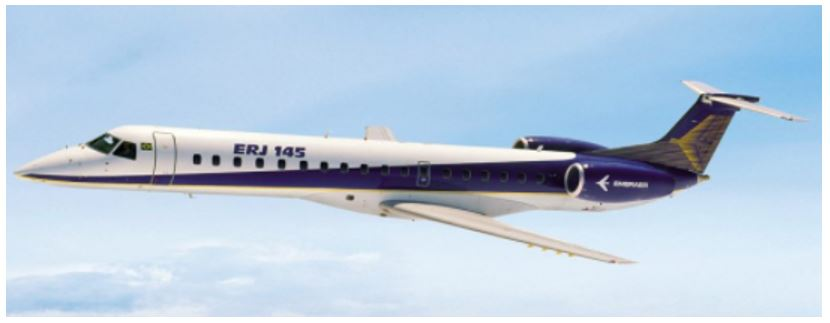
\includegraphics[width=1\textwidth]{pesquisademercado/EmbraerERJ145.jpg}
\caption{Embraer~ERJ145}
\end{figure}

\begin{table}
\centering
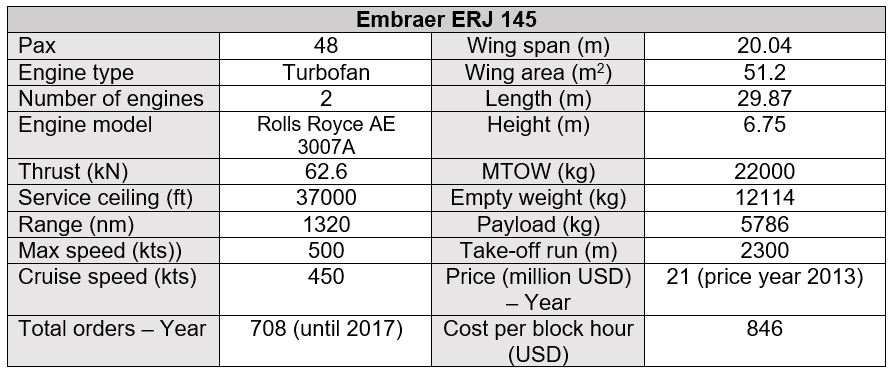
\includegraphics[width=0.9\textwidth]{pesquisademercado/tabelaEmbraerERJ145.jpg}
\caption{Características do Embraer~ERJ145}
\end{table}

\begin{sidewaysfigure}[p]
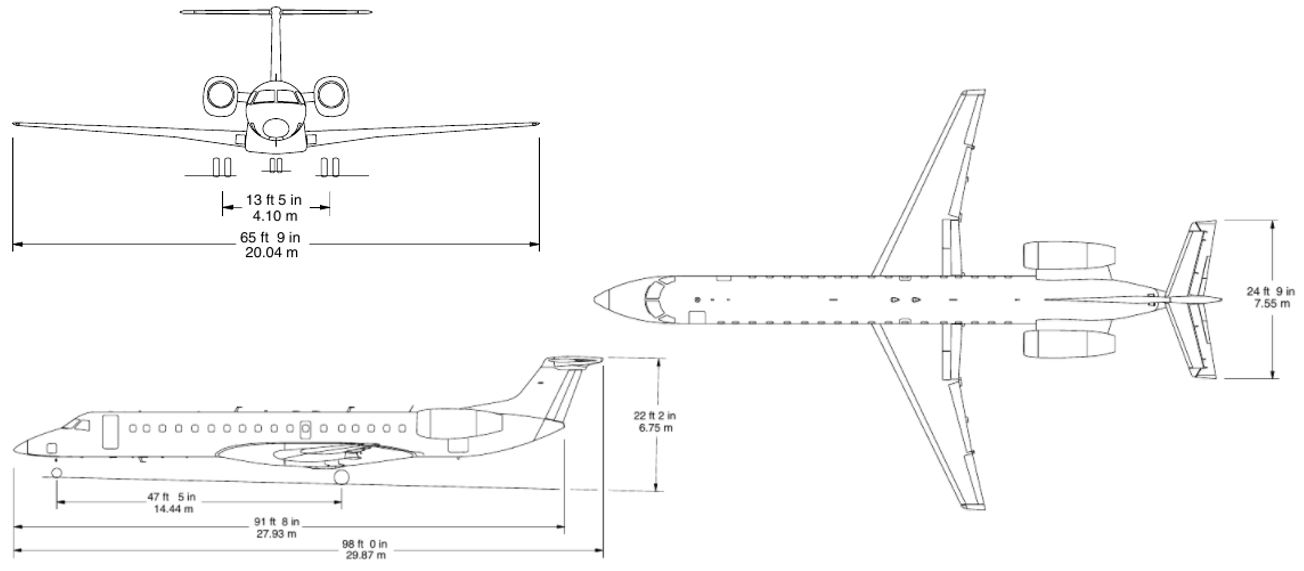
\includegraphics[width=\textwidth]{pesquisademercado/dimensoesExternasEmbraerERJ145.jpg}
\caption{Três vistas do Embraer~ERJ145}
\end{sidewaysfigure}

\begin{sidewaysfigure}[p]
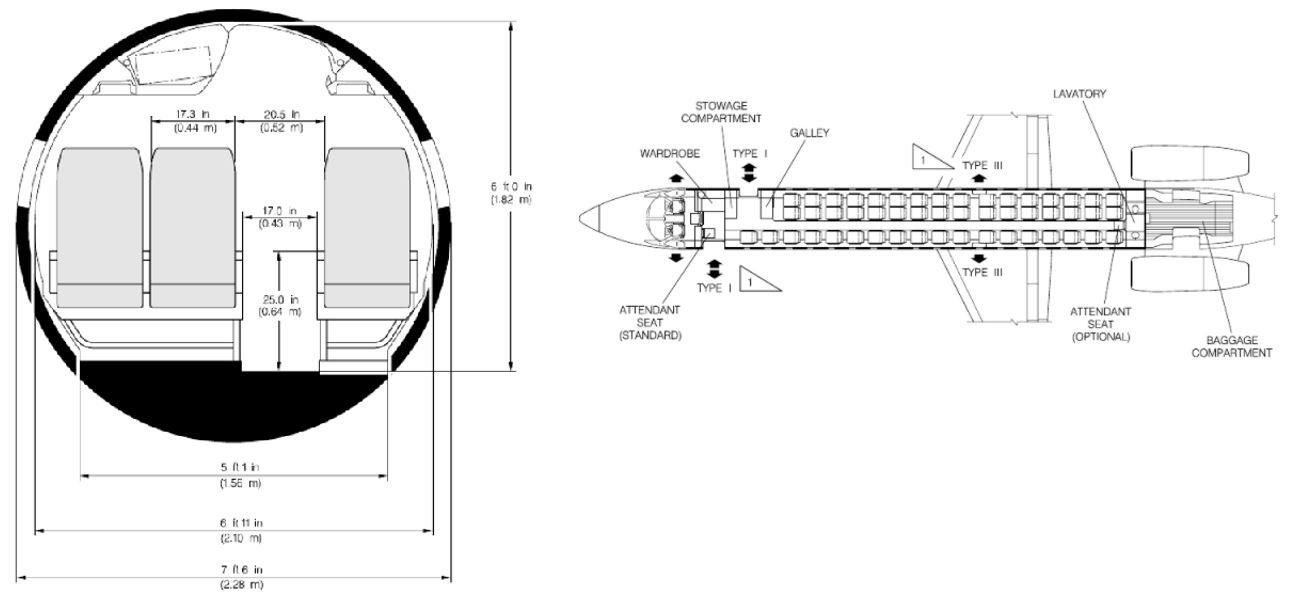
\includegraphics[width=\textwidth]{pesquisademercado/dimensoesInternasEmbraerERJ145.jpg}
\caption{Seção transversal e longitudinal (LOPA) do Embraer~ERJ145}
\end{sidewaysfigure}

\clearpage
%\subsection{Embraer E 170}
\begin{figure}
\centering
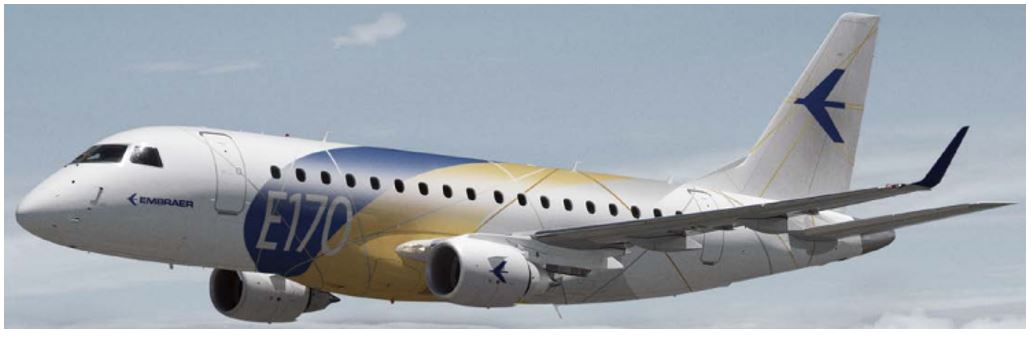
\includegraphics[width=1\textwidth]{pesquisademercado/EmbraerE170.jpg}
\caption{Embraer~E170}
\end{figure}

\begin{table}
\centering
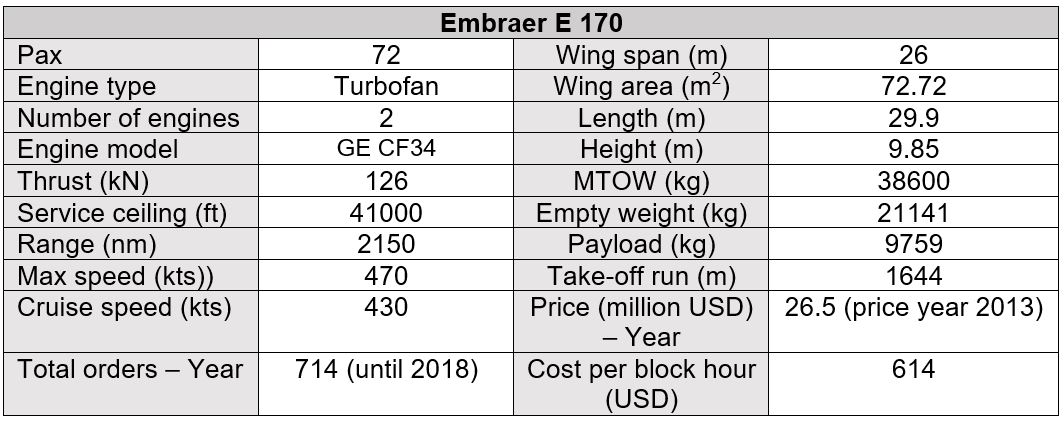
\includegraphics[width=0.9\textwidth]{pesquisademercado/tabelaEmbraerE170.jpg}
\caption{Características do Embraer~E170}
\end{table}

\begin{sidewaysfigure}[p]
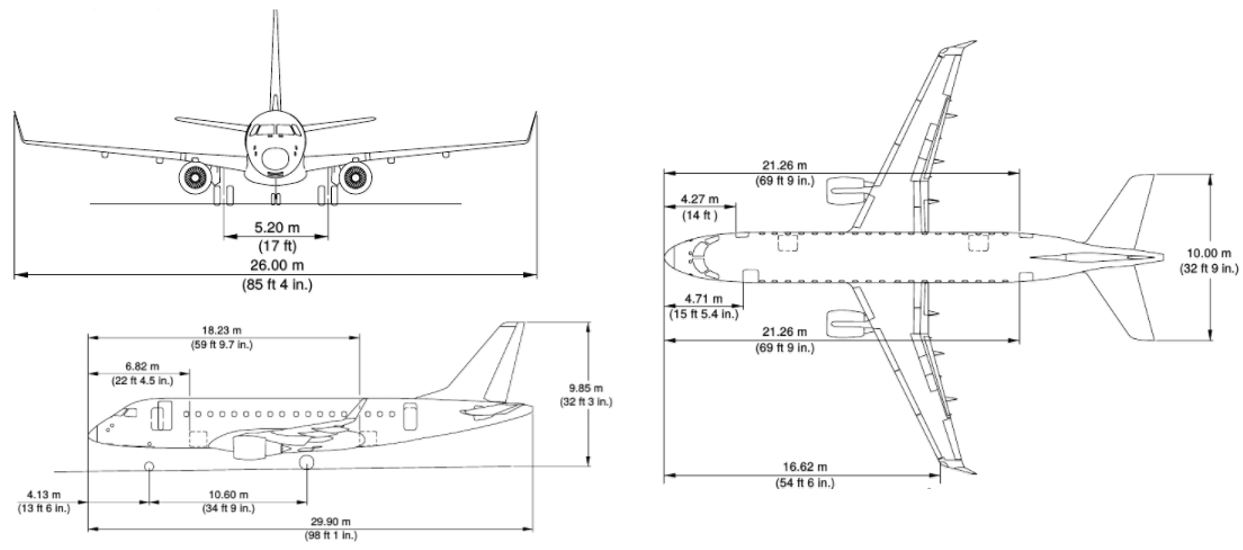
\includegraphics[width=\textwidth]{pesquisademercado/dimensoesExternasEmbraerE170.jpg}
\caption{Três vistas do Embraer~E170}
\end{sidewaysfigure}

\begin{sidewaysfigure}[p]
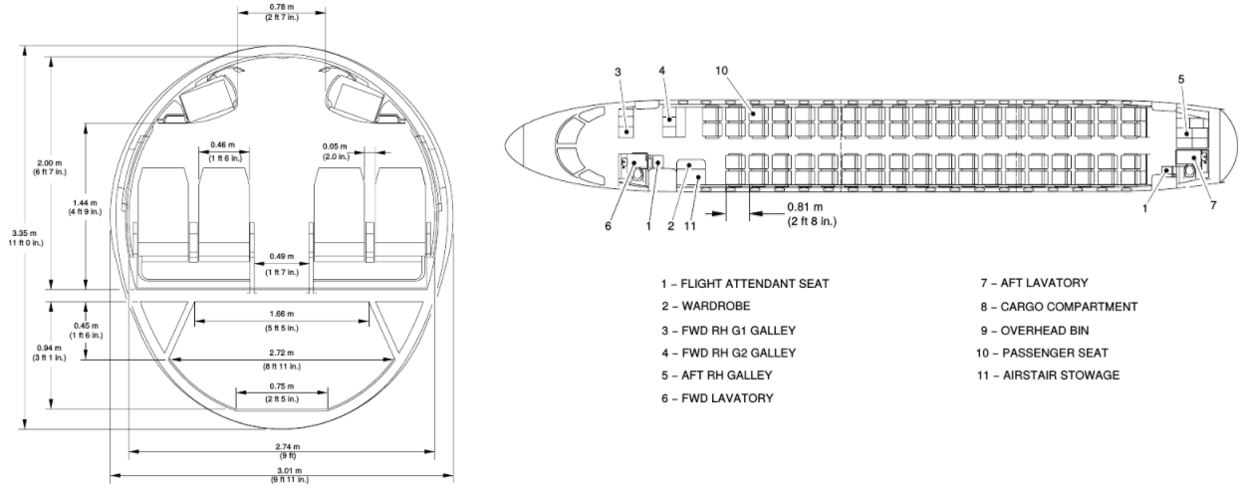
\includegraphics[width=\textwidth]{pesquisademercado/dimensoesInternasEmbraerE170.jpg}
\caption{Seção transversal e longitudinal (LOPA) do Embraer~E170}
\end{sidewaysfigure}

\clearpage
%\subsection{Bombardier Dash 8}
\begin{figure}
\centering
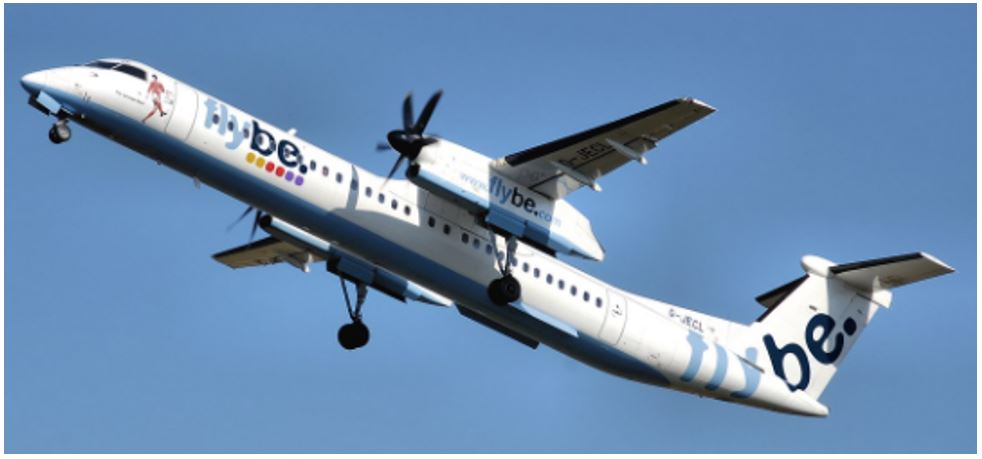
\includegraphics[width=1\textwidth]{pesquisademercado/BombardierDash8.jpg}
\caption{Bombardier~Dash~8}
\end{figure}

\begin{table}
\centering
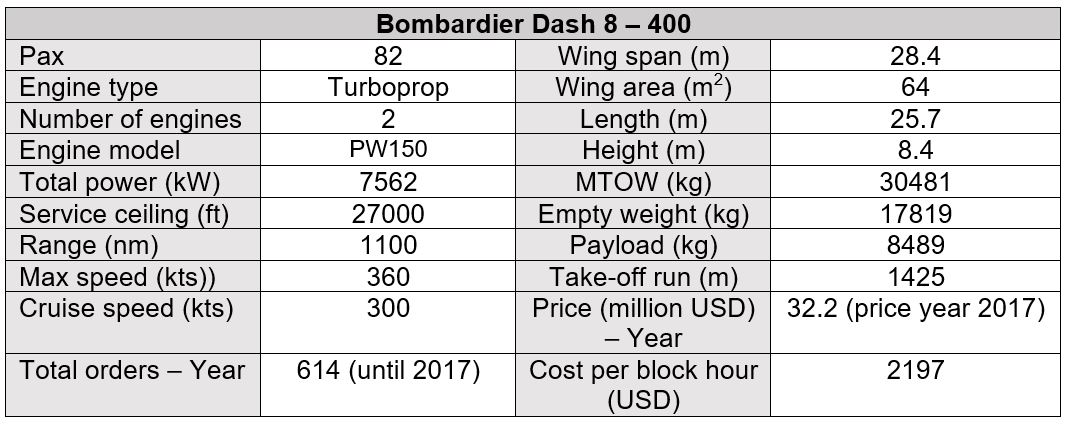
\includegraphics[width=0.9\textwidth]{pesquisademercado/tabelaBombardierDash8.jpg}
\caption{Características do Bombardier~Dash~8}
\end{table}

\begin{sidewaysfigure}[p]
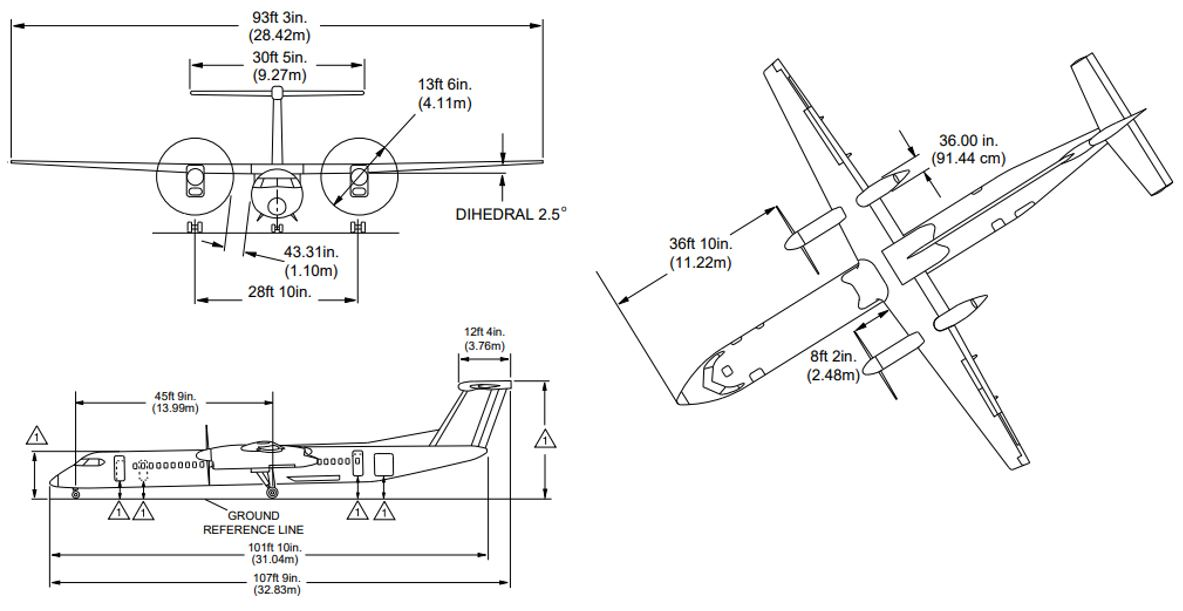
\includegraphics[width=\textwidth]{pesquisademercado/dimensoesExternasBombardierDash8.jpg}
\caption{Três vistas do Bombardier~Dash~8}
\end{sidewaysfigure}

\begin{sidewaysfigure}[p]
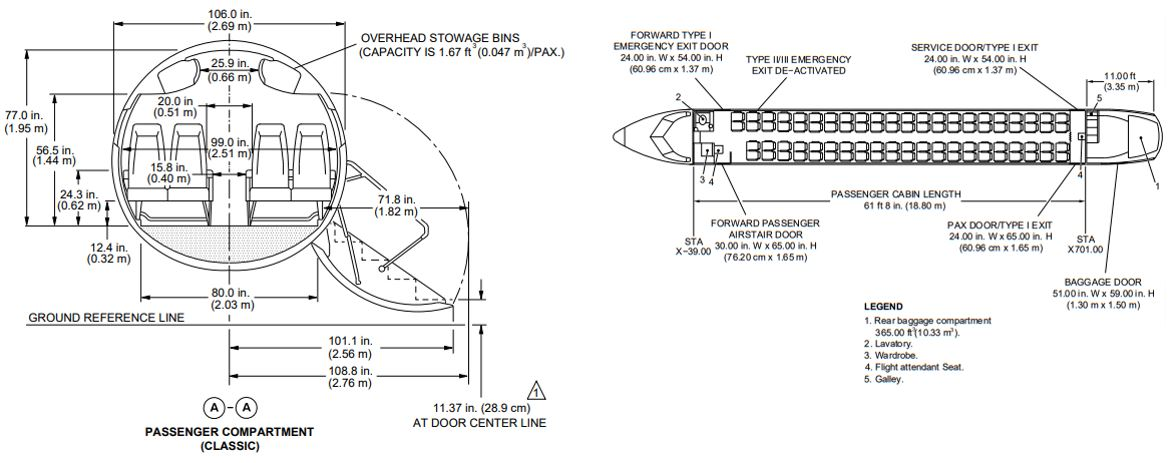
\includegraphics[width=\textwidth]{pesquisademercado/dimensoesInternasBombardierDash8.jpg}
\caption{Seção transversal e longitudinal (LOPA) do Bombardier~Dash~8}
\end{sidewaysfigure}

\clearpage
%\subsection{ATR 42}
\begin{figure}
\centering
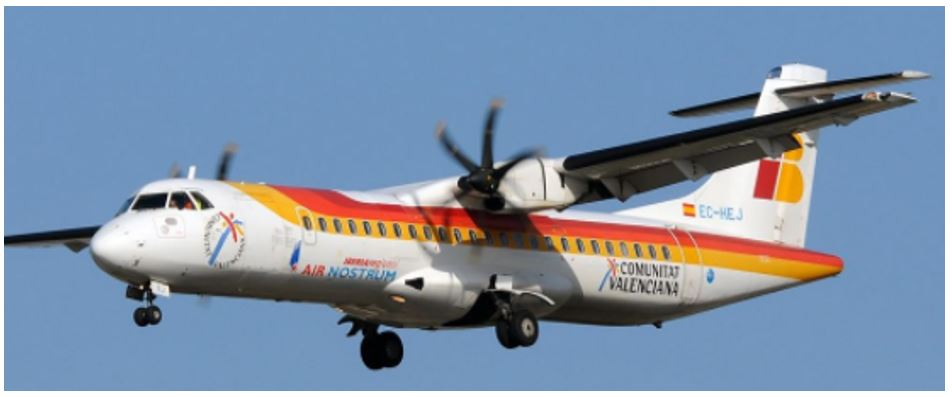
\includegraphics[width=1\textwidth]{pesquisademercado/ATR42.jpg}
\caption{ATR~42-300}
\end{figure}

\begin{table}
\centering
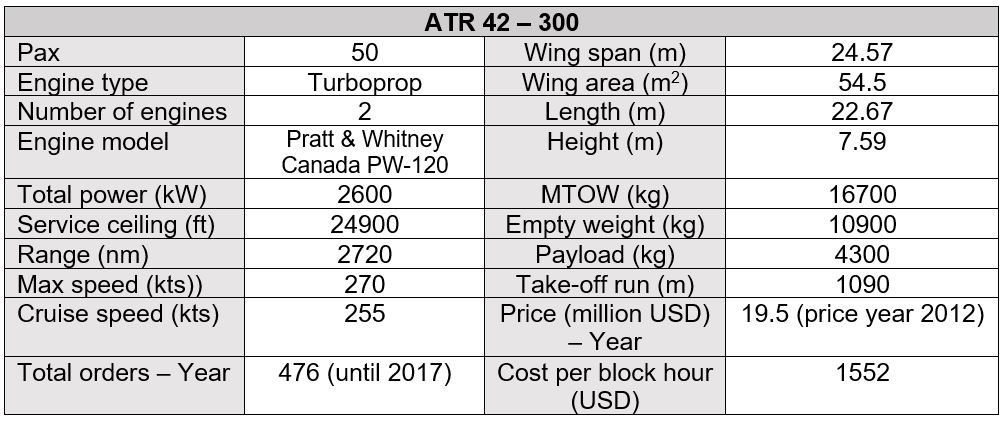
\includegraphics[width=0.9\textwidth]{pesquisademercado/tabelaATR42.jpg}
\caption{Características do ATR~42-300}
\end{table}

\begin{sidewaysfigure}[p]
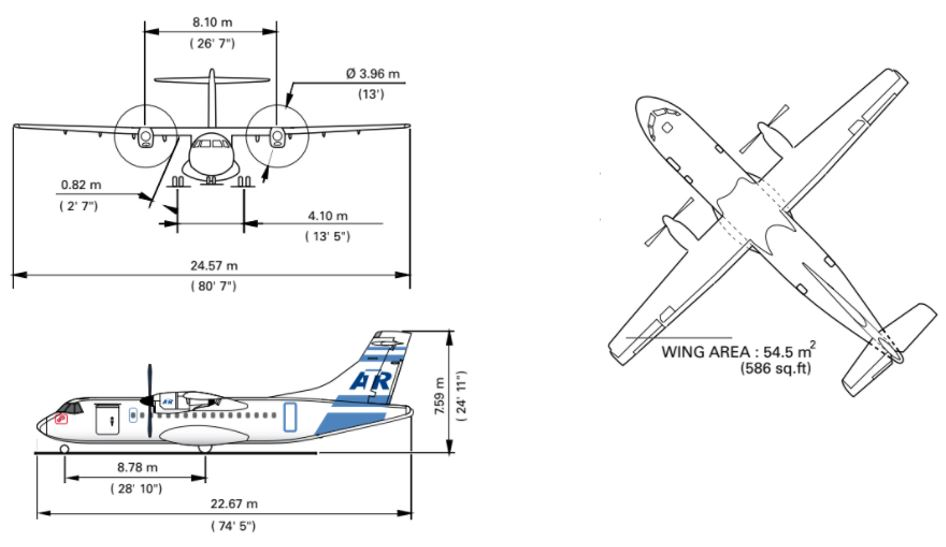
\includegraphics[width=\textwidth]{pesquisademercado/dimensoesExternasATR42.jpg}
\caption{Três vistas do ATR~42-300}
\end{sidewaysfigure}

\begin{sidewaysfigure}[p]
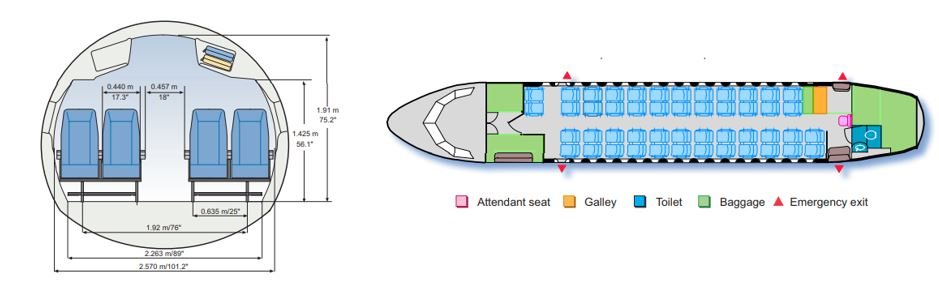
\includegraphics[width=\textwidth]{pesquisademercado/dimensoesInternasATR42.jpg}
\caption{Seção transversal e longitudinal (LOPA) do ATR~42-300}
\end{sidewaysfigure}

\clearpage
%\subsection{Embraer EMB-120}
\begin{figure}
\centering
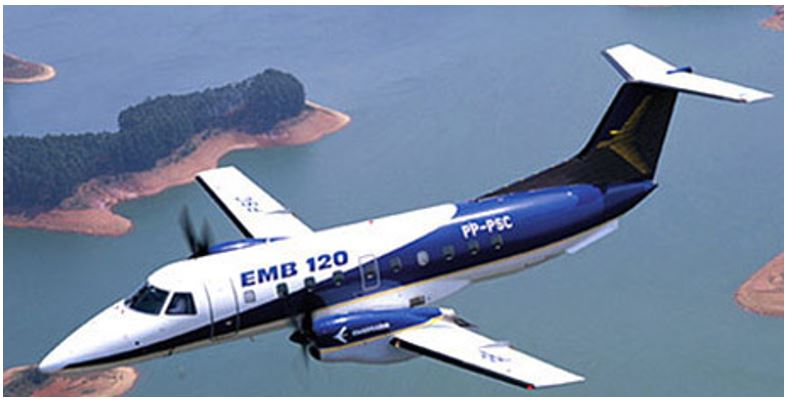
\includegraphics[width=1\textwidth]{pesquisademercado/EmbraerEMB120.jpg}
\caption{Embraer~EMB120}
\end{figure}

\begin{table}
\centering
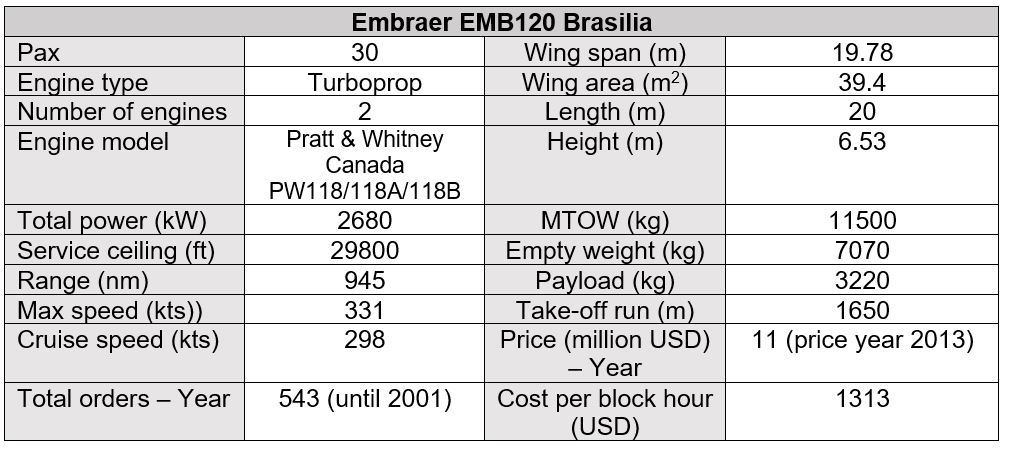
\includegraphics[width=0.9\textwidth]{pesquisademercado/tabelaEmbraerEMB120.jpg}
\caption{Características do Embraer~EMB120}
\end{table}

\begin{sidewaysfigure}[p]
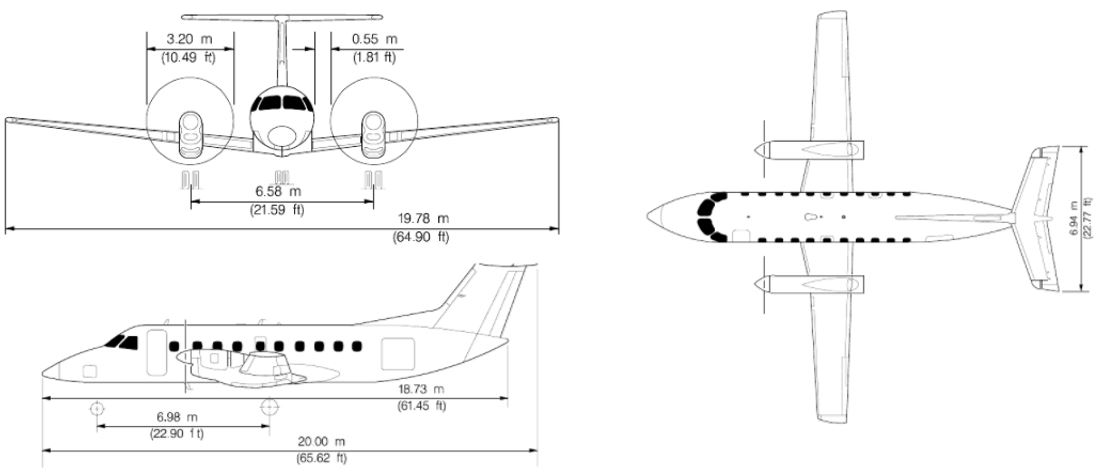
\includegraphics[width=\textwidth]{pesquisademercado/dimensoesExternasEmbraerEMB120.jpg}
\caption{Três vistas do Embraer~EMB120}
\end{sidewaysfigure}

\begin{sidewaysfigure}[p]
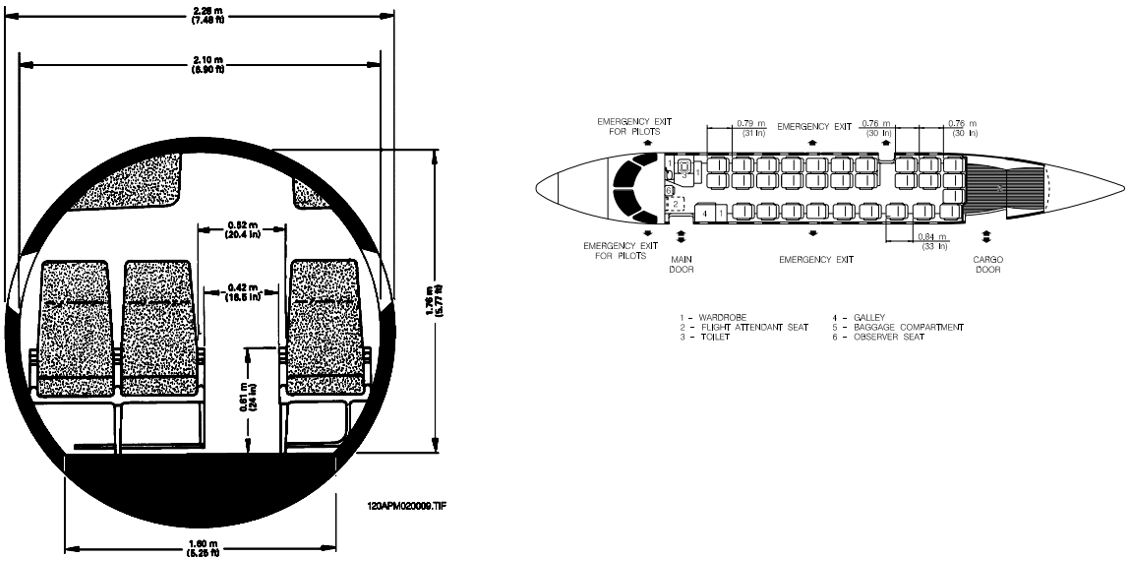
\includegraphics[width=\textwidth]{pesquisademercado/dimensoesInternasEmbraerEMB120.jpg}
\caption{Seção transversal e longitudinal (LOPA) do Embraer~EMB120}
\end{sidewaysfigure}
